% !TeX encoding = UTF-8
% !TeX spellcheck = en_US
% !TeX root = ../../Thesis.tex

\chapter{Vacuum test chamber}
\label{ch:Vacuum chamber}

Since the QUAK experiment will use cold potassium atoms, a vacuum chamber is necessary. The goal of our preliminary setup was to only test and characterize the electron beam without the presence of trapped atoms. Low pressure is necessary to provide a mean free path long enough so that electrons do not scatter too much. It was important to characterize the electron beam with a phosphor coated CRT screen inside our chamber. Therefore CF160 flanges were chosen. 


\section{Chamber Setup}
\label{sec:Chamber Setup}

A 3D render of the chamber is shown in (\cref{fig:3D rendering of test chamber}). The center piece consists of a 6-way cross with view ports at the front and bottom. A valve was installed at the back in order to flood the chamber with nitrogen (Alphagaz\texttrademark,~N$_2$ purity $\ge\SI{99.999}{\percent}$) when inserting a new CRT to avoid water vapor and oxygen getting into the chamber. On the right side, a HiCube 300 Eco turbo pump was connected. To the left, a wobble stick was inserted with a wire to move items inside the closed chamber. Later, a Faraday cup was attached to it (see \cref{sec:Faraday cup} for more information). A straight CF160 pipe of length \SI{27}{\centi\meter} was put at the top with a 5 port cluster flange, each being of type CF40.
 
In the middle port, a Thyracont VSH89DL pressure gauge was installed. On the left, a MIL 19 C connector was set up to supply the necessary voltages to the CRT. Two flanges were equipped with four BNC feedthroughs each. One of them was used to connect the x-, and y-plates, while the other connected to the wobble stick and aluminum foil at the CRT screen. Further explanation will be given in \cref{ch:Beam Characterization}. The last port was capped off by a blank flange.
 
For wires inside the chamber, at first stranded copper cables were used. These were later swapped for Kapton insulated BNC cables. The chamber was sealed by Viton rubber gaskets which were changed to copper gaskets. Only the gasket at the cluster flange was kept to rubber since the chamber was opened and closed multiple times at that connection.
 
\begin{figure}[ht]
	\centering
 	
	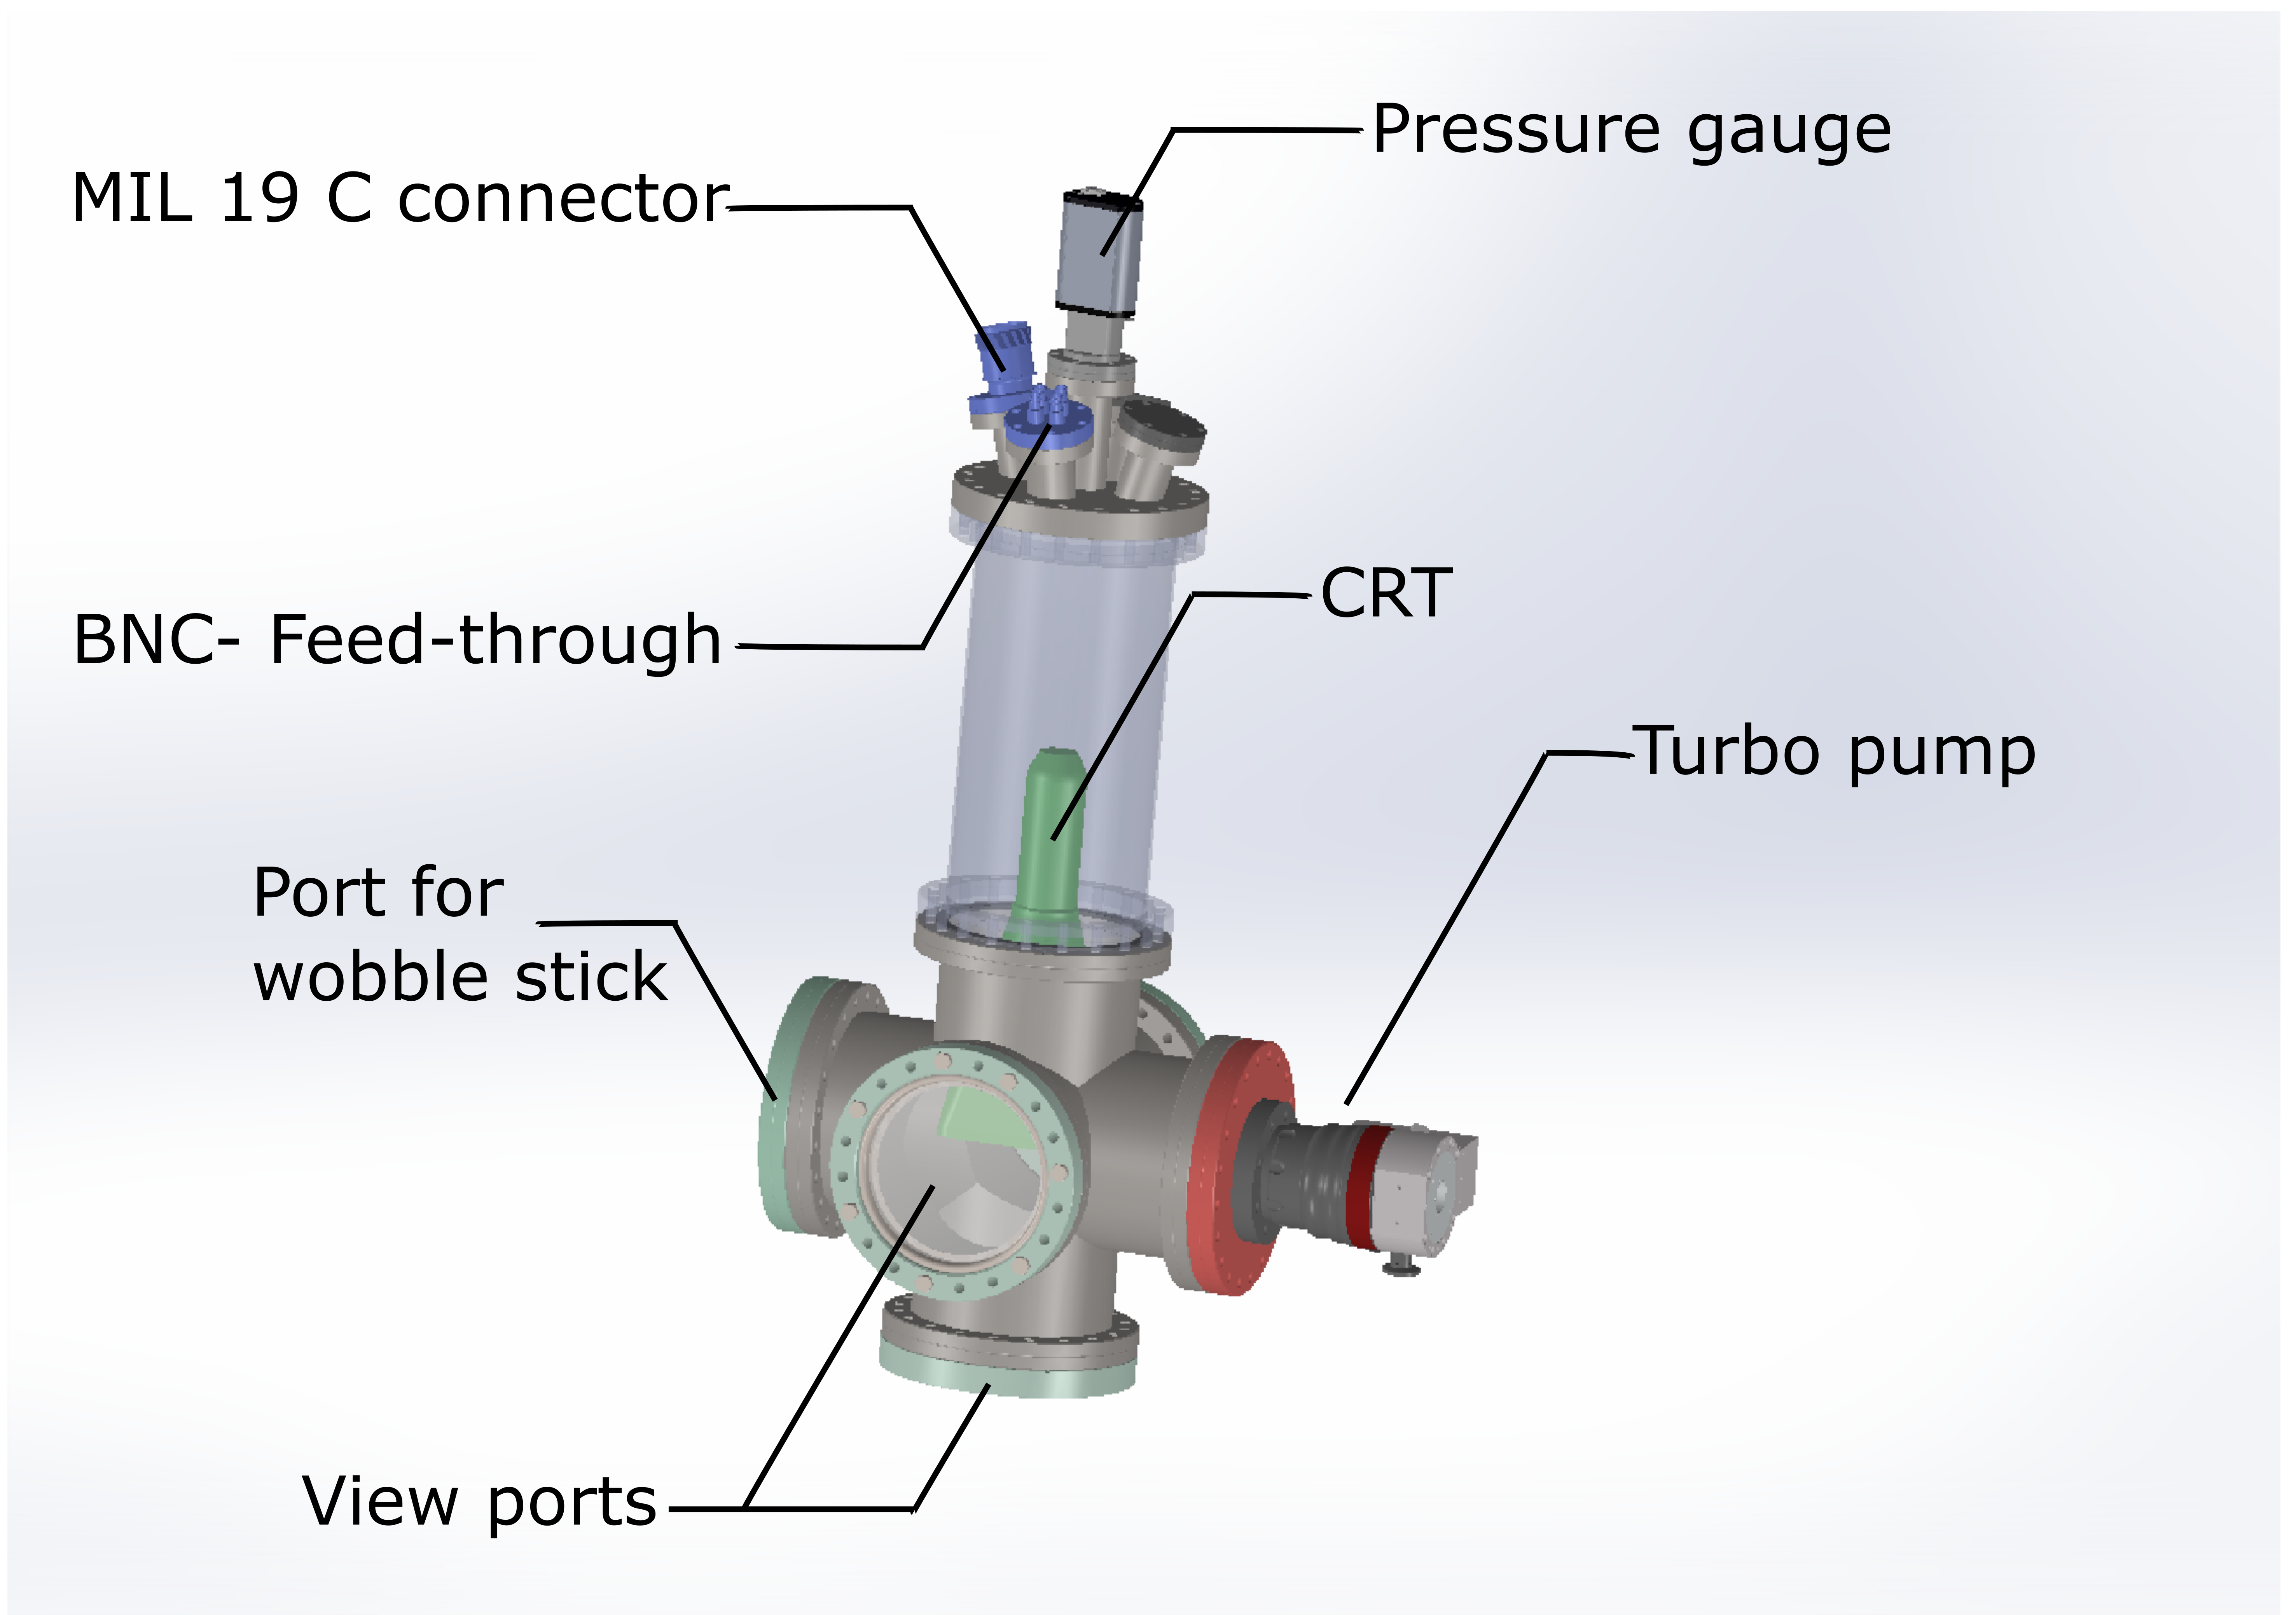
\includegraphics[width=0.9\textwidth]{./Chapters/vacuum-chamber/vacuum-chamber-annotated} % taken from OneNote QuaK/Vacuum Setup/Test vacuum chamber
	
	\caption{3D rendering of test chamber.}
	\label{fig:3D rendering of test chamber}
\end{figure}
 
\subsection{CRT mounting mechanism}
\label{subsec:CRT mounting mechanism}

Two M8 rods of length \SI{66}{\centi\meter} were screwed with a counter nut into the cluster flange. On each, a L shaped aluminum piece was installed between two nuts. These were then connected by a hose clamp, which was used to secure the CRT inside below the cluster flange (\cref{fig:Image of CRT mounting mechanism}).
 

\begin{figure}[ht]
	\centering
	
	\includegraphics[width=.9\textwidth]{Chapters/vacuum-chamber/Mounting.JPG}
	%\missingfigure[figwidth=0.9\textwidth]{Image of CRT mounting mechanism.}
	
	\caption{Image of CRT mounting mechanism.}
	\label{fig:Image of CRT mounting mechanism}
\end{figure}


\section{Leak-testing the vacuum test chamber}
\label{sec:Leak-testing the vacuum test chamber}

Before inserting a CRT for the first time, measurements were made in order to find out how well low pressure could be maintained inside the setup. First, the chamber was set to a pressure of \SI{e-5}{\milli\bar} after which the pump was turned off. The pressure was measured once a minute for a duration \SI{3}{\hour}. This is shown in \cref{fig:Time evolution of pressure inside the test chamber after turning off pump}.

\begin{figure}[ht]
	\centering
		
	\begin{tikzpicture}
		% !TeX encoding = UTF-8
% !TeX spellcheck = en_US
% !TeX root = ../../Thesis.tex

\begin{axis}[
	%name=zeemanShift,
	%grid=major,
	ymode = log,
	xlabel = time/\si{\minute},
	ylabel = pressure/\si{\milli\bar},
	%scaled ticks=false,
	%		every x tick scale label/.style={at={(xticklabel* cs:1.03,-0.3em)}, /pgfplots/near ticklabel align=outside, anchor=near xticklabel opposite, inner sep=0pt},
	%		xticklabel style={/pgf/number format/sci}, sci generic={mantissa sep=\cdot,exponent={10^{#1}}}},
	%yticklabel style={/pgf/number format/sci},
	xmin = 0,
	ymin = 1e-5,
	%extra tick style={grid=none}, 
	%width=0.7\textwidth,
	%legend style={at={(1.02, 0.5)}, anchor = west},
	%every axis plot/.append style={thick}
	]
	\addplot[mark=none, black] table [x=t, y=p, col sep=comma]{./Chapters/vacuum-chamber/leak_rate.csv};
\end{axis}
	\end{tikzpicture}
	
	\caption{Time evolution of pressure inside the test chamber after turning off pump.}
	\label{fig:Time evolution of pressure inside the test chamber after turning off pump}
\end{figure}

Without a CRT installed, it was possible to reach a pressure of \SI{6.8e-7}{\milli\bar}. With a CRT installed inside, the lowest achieved pressure was \SI{2.0e-6}{\milli\bar}. It was not possible to reach a lower pressure due to outgassing. As mentioned in \cref{sec:Chamber Setup}, changes were made to the chamber. Thanks to these, it was possible to reach a pressure of \SI{1.2e-7}{\milli\bar} with a CRT inside the setup.

\section{CF-Flange Fastening Method}
\label{sec:CF-Flange fastening method}

When attaching flanges, it is important to start with a low torque and to fasten opposite screws to prevent too much force on one side of the gasket. For M6 screws, the torque was incrementally set to \SIlist{6;10;15;20}{\newton\meter} and for M8 screws \SIlist{8;16;25}{\newton\meter}. After finishing every opposite screw pair at a set torque, the procedure was repeated twice before going to a higher torque. This was done in order guarantee a tight and even seal.